\documentclass{beamer}
%
% Choose how your presentation looks.
%
% For more themes, color themes and font themes, see:
% http://deic.uab.es/~iblanes/beamer_gallery/index_by_theme.html
%
\mode<presentation>
{
  \usetheme{default}      % or try Darmstadt, Madrid, Warsaw, ...
  \usecolortheme{default} % or try albatross, beaver, crane, ...
  \usefonttheme{default}  % or try serif, structurebold, ...
  \setbeamertemplate{navigation symbols}{}
  \setbeamertemplate{caption}[numbered]
} 

\usepackage[english]{babel}
\usepackage[utf8]{inputenc}
\usepackage[T1]{fontenc}

\title[Conicas]{Cônicas}
\author{MAP 2110 - Diurno}
\institute{IME USP}
\date{14 de abril}

\begin{document}

\begin{frame}
  \titlepage
\end{frame}

% Uncomment these lines for an automatically generated outline.
%\begin{frame}{Outline}
%  \tableofcontents
%\end{frame}


\section{Cônicas}

\begin{frame}{Seções cônicas}

  Cônicas são curvas planas estudadas desde a antiga Grécia e que possuem muitas
  propriedades de interesse, principalmente na física. A parte, talvez, mais 
  importante historicamente é a prova de que a trajetória dos planetas em torno do 
  Sol é uma elipse. Formulada por Kepler, esta hipótese foi posteriormente provada
  por Newton. Quais propriedades são as mais interessantes? A resposta determina 
  qual será a definição usada para nosso objeto.

  
\end{frame}

\begin{frame}{Definição}
  O Apostol apresenta três possíveis definições de cônicas, e todos são equivalentes.
  Mas vamos usar a definição que faz mais uso do conceito de vetor, e coordenadas.
  Como as cônicas estão num plano podemos fazer todas as contas em $V_2$.

  \textbf{Definição:} Se $L$ é uma reta em $V_2$, $F$ é um ponto fora de $L$ e $e>0$ um 
  número real positivo, então o conjunto:
  $$ C=\{X : \|X-F\| = e d(X,L)    \}$$ é uma cônica, e diremos que $C$ é uma elípse se 
  $e<1$, uma parábola se $e=1$ e uma hipérbole se $e>1$

  % figura aqui ou slide com figura

\end{frame}

\begin{frame}{Como expressar $d(X,L)$}
 Nosso primeiro problema (exercício) é: Dado ponto qualquer $P$ da reta $L$ e 
 $N$ um vetor unitário, ortogonal à $L$, mostre que $d(x,L)=|(X-P)\cdot N|$
\end{frame}
\begin{frame}

  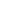
\includegraphics{reta1.png}

\end{frame} 

\begin{frame}

  Escrevemos:
  \begin{gather*}
    X-P = X-Q + Q-P \\
    X-P = \pm d(X,L)N+ Q-P \implies \\
    (X-P)\cdot N = \pm d(X,L) 
  \end{gather*}
\end{frame}


\begin{frame}

  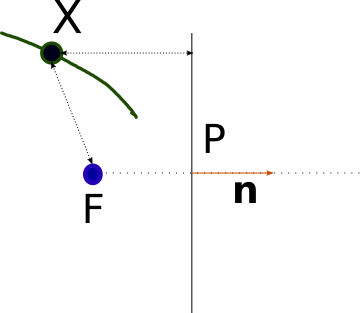
\includegraphics{conica1.png}
\end{frame}

\begin{frame}
Na figura, $\mathbf{n}$ é um vetor unitário apontando para o lado contrário de $F$
Então temos:
\begin{gather*}
  F-P = -d\mathbf{n} \text{ } d>0 \text{ e } F-P = (F-X) + (X-P) \\
  (F-P)\cdot \mathbf{n}= (F-X)\cdot \mathbf{n} + (X-P)\cdot \mathbf{n}\\
  -d = -(X-F)\cdot\mathbf{n} -d(X,L) \implies d(X,L)=|(X-F)\cdot\mathbf{n}-d|
  \end{gather*}
  Isto dá uma forma equivalente de definir a cônica onde não aparece diretamente a reta 
  diretriz!
  $$\|X-F\| = e |(X-F)\cdot\mathbf{n}-d|$$
\end{frame}

    \begin{frame}{Equações polares }
     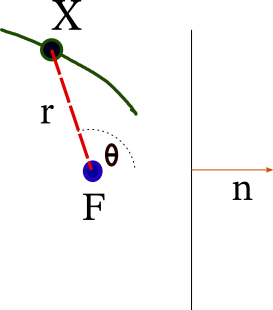
\includegraphics{conica2.png}
    \end{frame}
   
    \begin{frame}{}
     \begin{gather*}
       \|X-F\| = r \text{ } (X-F)\cdot\mathbf{n} = r\cos(\theta)\\
       r= e|r\cos(\theta) - d|
     \end{gather*}
      
    \end{frame}
    \begin{frame}{}
      Se $r\cos(\theta)-d <=0 $ então $|r\cos(\theta)-d |=d -r\cos(\theta)$
      e a equação da cônica fica
      $$ r = \frac{ed}{1+e\cos{\theta}}$$
      No outro caso, se $r\cos(\theta)-d >0$ teremos
      $$ r= \frac{ed}{e\cos{\theta}-1}$$
      claramente isso só ocorre se $e>1$, ou seja,
      só na hipérbole. 
    \end{frame}
\begin{frame}
  
\end{frame}
\begin{frame}{Equações cartesianas} 
  Voltando às equações de definição das cônicas
  $$ \|X-F\| = e |(X-F)\cdot\mathbf{n}-d|$$ 
  Vamos assumir que temos simetria em relação à origem e elevar os lados ao quadrado.
  \begin{gather*}
    (X-F)^2 = e^2((X-F)\cdot\mathbf{n}-d)^2\\
    \|X\|^2 -2X\cdot F + \|F\|^2 = e^2(X.\cdot \mathbf{n})^2 + 2ea(X.\cdot \mathbf{n})
    + a^2\\
    a = ed + e F\cdot\mathbf{n}\\
    \text{ usando a simetria teremos} \\
    \|X\|^2 + e^2a^2 =e^2(X.\cdot \mathbf{n})^2+a^2
  \end{gather*}
\end{frame}

\begin{frame}{Exercício 1}
   fazer o esboço da curva:
   \begin{gather*}
     r= \frac{2}{1+\cos{\theta}} \\
     r = \frac{3}{1+0.5\cos(\theta)}
   \end{gather*}
  
\end{frame}
\begin{frame}
  No primeiro caso temos uma paràbola ($e=1$), com $d=2$, e no segundo caso uma elipse ($e=0.5$)
  com $d=6$
  
\end{frame}

\begin{frame}
  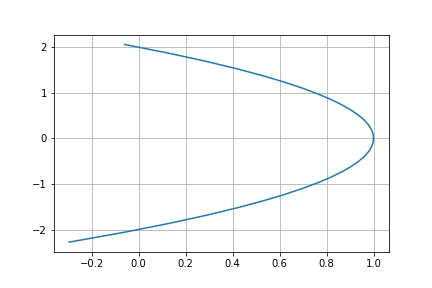
\includegraphics{coni1.png}
\end{frame}  

\begin{frame}
  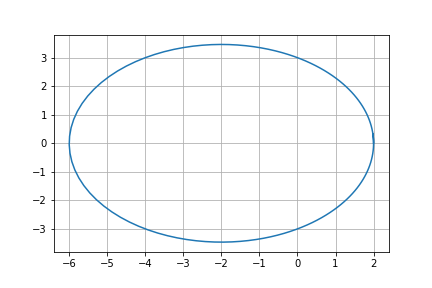
\includegraphics{coni2.png}
\end{frame} 


\begin{frame}
  Achar a equação polar da cônica com $e=1/2$ e diretriz $3x+4y=25.$ (Foco em $(0,0)$)
  
\end{frame}

\begin{frame}
  A reta diretriz passa por $(3,4)$, e também $(3,4)$ é um vetor normal à diretriz. Temos então que
  $d=5 =\|(3,4)\|$ como $e=0.5$ a equação polar fica
  $$ r = \frac{2.5}{1+0.5*\cos(\theta-\theta_0)}$$

  
\end{frame}
A reta diretriz passa por $(3,4)$, e também $(3,4)$ é um vetor normal à diretriz. Temos então que
$d=5 =\|(3,4)\|$ como $e=0.5$ a equação polar fica
$$ r = \frac{2.5}{1+0.5*\cos(\theta-\theta_0)}$$
Aqui $\theta_0$ é o ângulo que a reta normal à diretriz forma com $\mathbf{i}$, ou seja 
$\cos(\theta_0)=3/5.$


\end{document}
